\documentclass[12pt,a4paper]{article}

% ── Geometry & spacing ──────────────────────────────────────
\usepackage[margin=2.5cm]{geometry}
\setlength{\headheight}{14.5pt}
\addtolength{\topmargin}{-2.5pt}
\setlength{\parindent}{1.25em}
\setlength{\parskip}{0pt}

% ── Encoding & language ─────────────────────────────────────
\usepackage[T1]{fontenc}
\usepackage[utf8]{inputenc}
% Swap the two lines below to switch language:
% \usepackage[english]{babel}       
\usepackage[indonesian]{babel}     % Bahasa Indonesia

% ── Font ────────────────────────────────────────────────────
\usepackage{lmodern}

% ── Math ────────────────────────────────────────────────────
\usepackage{amsmath, amssymb, amsthm}
\usepackage{mathtools}

% ── Graphics & figures ──────────────────────────────────────
\usepackage{graphicx}
\usepackage{float}
\usepackage{caption}
\usepackage{subcaption}

% ── Tables ──────────────────────────────────────────────────
\usepackage{booktabs}
\usepackage{array}
\usepackage{longtable}

% ── Lists ───────────────────────────────────────────────────
\usepackage{enumitem}

% ── Code listings ───────────────────────────────────────────
\usepackage{listings}
\usepackage{xcolor}

\definecolor{codebg}{RGB}{245,245,245}
\definecolor{codeframe}{RGB}{200,200,200}
\definecolor{codekw}{RGB}{0,0,180}
\definecolor{codecomment}{RGB}{60,128,49}
\definecolor{codestring}{RGB}{163,21,21}

\lstdefinestyle{default}{
  backgroundcolor=\color{codebg},
  basicstyle=\ttfamily\small,
  breaklines=true,
  breakatwhitespace=false,
  tabsize=2,
  showstringspaces=false,
  frame=single,
  rulecolor=\color{codeframe},
  numbers=left,
  numberstyle=\tiny\color{gray},
  numbersep=8pt,
  xleftmargin=2.5em,
  framexleftmargin=2em,
  keywordstyle=\color{codekw}\bfseries,
  commentstyle=\color{codecomment}\itshape,
  stringstyle=\color{codestring},
}
\lstdefinestyle{go}{style=default, language=Python}    % closest builtin
\lstdefinestyle{python}{style=default, language=Python}
\lstdefinestyle{java}{style=default, language=Java}
\lstdefinestyle{cpp}{style=default, language=C++}
\lstdefinestyle{bash}{style=default, language=bash}

\lstset{style=default}   % global default

% ── Boxes (for tips / callouts) ──────────────────────────────
\usepackage{tcolorbox}
\tcbuselibrary{listings, skins, breakable}

\newtcolorbox{infobox}[1][Note]{
  colback=blue!5!white, colframe=blue!50!black,
  fonttitle=\bfseries, title=#1,
  breakable
}
\newtcolorbox{warnbox}[1][Warning]{
  colback=orange!10!white, colframe=orange!80!black,
  fonttitle=\bfseries, title=#1,
  breakable
}

% ── Hyperlinks ──────────────────────────────────────────────
\usepackage{hyperref}
\hypersetup{colorlinks=true, linkcolor=black, urlcolor=blue, citecolor=black}

% ── SI units ────────────────────────────────────────────────
\usepackage{siunitx}

% ── Header / Footer ─────────────────────────────────────────
\usepackage{fancyhdr}
\pagestyle{fancy}
\fancyhf{}
\lhead{\CourseCode{} -- \CourseName}
\rhead{\thepage}

% ── First-line indent on all sections ───────────────────────
\usepackage{indentfirst}

\newcommand{\CourseCode}{IF2224}
\newcommand{\CourseName}{Teori Bahasa Formal dan Otomata}
\newcommand{\AssignmentTitle}{Laporan Tugas Besar}
\newcommand{\AssignmentSubtitle}{Milestone 1}
\newcommand{\Semester}{Semester II / 2025--2026}

% Team / group
\newcommand{\GroupName}{GTFOTBFO (HBB)}
\newcommand{\MemberA}{Nathanael Imandatua Manurung - 13524021}
\newcommand{\MemberB}{Nicholas Wise Saragih Sumbayak - 13524037}
\newcommand{\MemberC}{Kurt Mikhael Purba - 13524065}
\newcommand{\MemberD}{Rava Khoman Tuah Saragih - 13524107}


% Institution
\newcommand{\Lab}{Laboratorium Ilmu dan Rekayasa Komputasi}
\newcommand{\Program}{Teknik Informatika}
\newcommand{\Faculty}{Sekolah Teknik Elektro dan Informatika}
\newcommand{\University}{Institut Teknologi Bandung}

% Repository / deployment links (used in Appendix)
\newcommand{\RepoURL}{https://github.com/your-org/your-repo}
\newcommand{\DeployURL}{https://your-deployment-url.example.com}

\begin{document}

\begin{titlepage}
  \begin{center}
    \vspace*{1cm}
    {\Huge \textbf{\AssignmentTitle}}\\[0.4cm]
    {\Large \textsc{\CourseCode{} \CourseName}}\\[0.2cm]
    {\large \textsc{\AssignmentSubtitle}}\\[0.2cm]
    {\large \textsc{\Semester}}\\[2cm]

    
\includegraphics[height=7cm]{logo-itb.png}\\[2cm]

    {\large \textbf{Disusun oleh:}}\\[0.3cm]
    {\large
      \textbf{\GroupName}\\[0.25cm]
      \MemberA\\
      \MemberB\\
      \MemberC\\
      \MemberD\\
    }

    \vfill

    {\large \textsc{\Lab}}\\[0.15cm]
    {\large \textsc{Program Studi \Program}}\\[0.15cm]
    {\large \textsc{\Faculty}}\\[0.15cm]
    {\large \textsc{\University}}\\
  \end{center}
\end{titlepage}

\tableofcontents
\newpage

\section{Pendahuluan}

Bahasa Pemrograman diciptakan sebagai perantara komunikasi antara manusia yang
mengerti logika dan bahasa tingkat tinggi dengan komputer yang hanya dapat
mengerti bahasa mesin (\textit{machine code}). Tanpa adanya bahasa pemrograman,
manusia harus menuliskan instruksi komputer secara tingkat rendah kepada
komputer yang hanya mengerti 0 dan 1. Dalam hierarkinya, bahasa tingkat tinggi
(\textit{high-level}) dirancang agar lebih mendekati bahasa manusia, namun hal ini
menuntut proses transformasi yang berlapis agar dapat dipahami oleh CPU.

\begin{figure}[H]
\centering
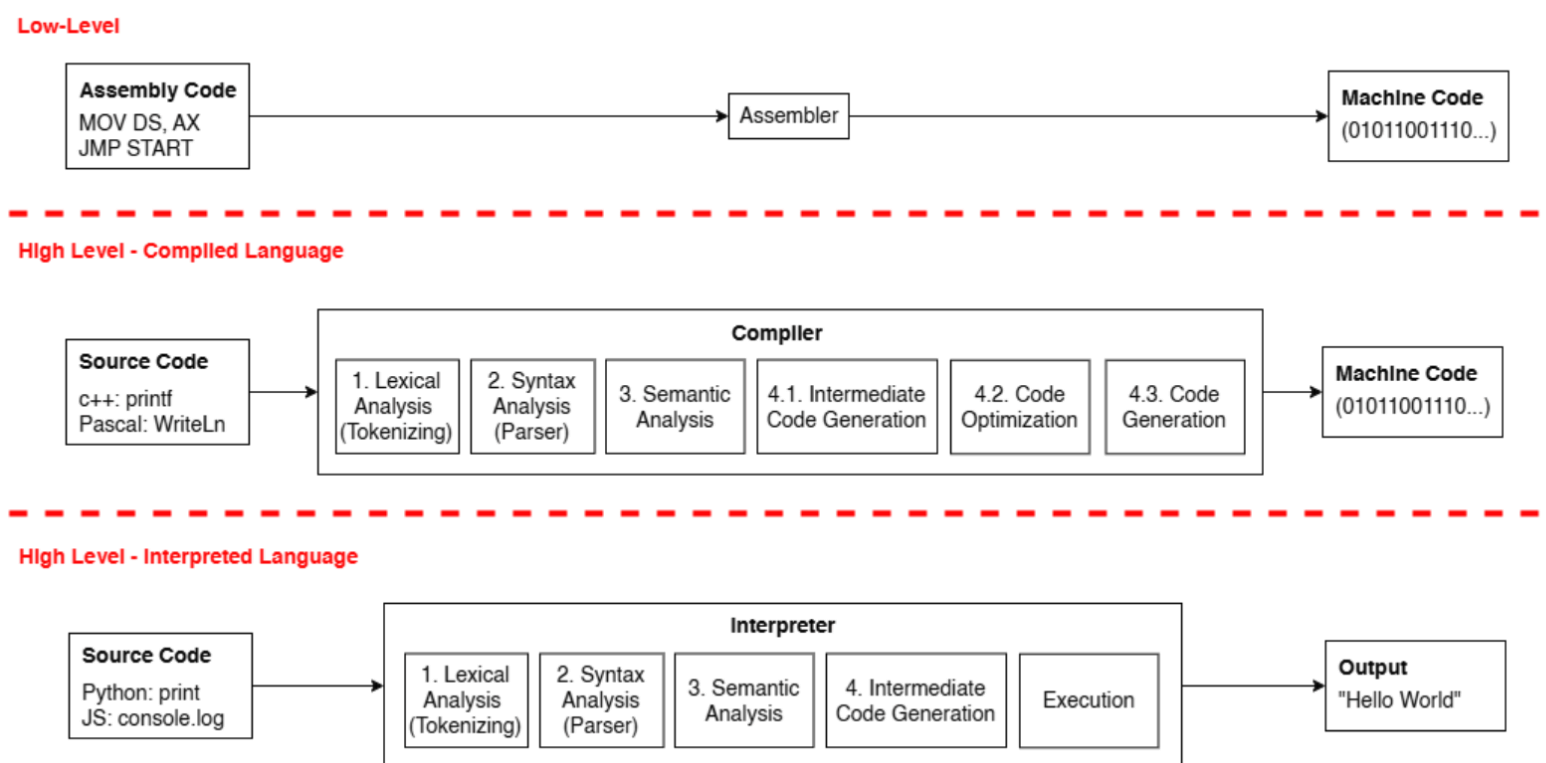
\includegraphics[width=0.8\textwidth]{tipe-bahasa.png}
\caption{Tipe-tipe bahasa pemrograman}
\caption*{Sumber: Asisten IF2224}
\end{figure}

Proses transformasi ini dilakukan melalui mekanisme \textit{compiler} atau
\textit{interpreter}. Tahap awal dan fundamental dalam mekanisme tersebut adalah
Analisis Leksikal (\textit{Lexical Analysis}). Pada tahap ini, kode sumber yang berupa
rangkaian karakter mentah dibaca dan dikelompokkan menjadi satuan makna terkecil
yang disebut token, seperti kata kunci (\textit{keyword}), pengenal
(\textit{identifier}), operator, dan konstanta. Analisis leksikal berperan
krusial dalam menyederhanakan tugas tahap berikutnya, yaitu parsing, dengan
membuang elemen yang tidak relevan seperti spasi dan komentar, serta mendeteksi
simbol invalid sejak awal.


\section{Dasar Teori}

\subsection{Pendefinisian Bahasa Pemrograman}
Bahasa Pemrograman adalah cara manusia untuk dapat memberikan perintah
(\textit{instruction}) kepada sebuah komputer. Setiap bahasa pemrograman
memiliki kata kunci dan aturannya masing-masing serta makna dari kata-kata itu
yang disebut sintaks(\textit{syntax}) dan semantik (\textit{semantics}).
Input yang terdapat kesalahan pada tingkat sintaks berarti input tersebut tidak
valid untuk bahasa pemrograman tersebut, sedangkan kesalahan pada tingkat
semantik umumnya berbentuk kesalahan logika.

\subsubsection{Hierarki Bahasa Pemrograman}
Berdasarkan tingkat abstraksinya, bahasa pemrograman diklasifikasikan menjadi dua kategori utama:
\begin{itemize}
\item \textbf{\textit{Low-Level Language} (Bahasa Tingkat Rendah)}: Bahasa yang instruksinya mendekati arsitektur perangkat keras dan bahasa mesin (biner 0 dan 1). Contohnya adalah \textit{Assembly}, yang memerlukan \textit{Assembler} untuk menerjemahkan kode menjadi instruksi yang dapat dipahami CPU.
\item \textbf{\textit{High-Level Language} (Bahasa Tingkat Tinggi)}: Bahasa yang dirancang agar lebih mudah dibaca dan dipahami oleh manusia karena menggunakan kosakata yang menyerupai bahasa natural. Semakin tinggi tingkat bahasa tersebut, semakin banyak tahapan pemrosesan yang diperlukan untuk mengubahnya menjadi kode mesin. Contoh bahasa tingkat tinggi antara lain Pascal, C++, Python, dan Java.
\end{itemize}

\subsubsection{\textit{Compiler} dan \textit{Interpreter} }
Untuk menjalankan kode sumber yang ditulis dalam bahasa tingkat tinggi,
diperlukan sebuah perangkat lunak penerjemah yang mengubah kode tersebut menjadi
format yang dapat dieksekusi oleh mesin. Secara umum, terdapat dua mekanisme
utama untuk mengubah bahasa tingkat tinggi ke bahasa mesin:

\begin{enumerate}
\item \textbf{\textit{Compiler} (Kompilator)}:
\textit{Compiler} adalah program yang menerjemahkan seluruh \textit{source code}
secara utuh menjadi kode mesin (biasanya dalam bentuk \textit{Object File})
sebelum program dijalankan. Proses kompilasi pada \textit{compiler} umumnya
terdiri dari empat tahapan utama: \textit{Lexical Analysis}, \textit{Syntax
Analysis}, \textit{Semantic Analysis}, dan \textit{Intermediate Code
Generation}. Karakteristik utama \textit{compiler} adalah jika terdeteksi adanya
kesalahan (\textit{error}) di dalam \textit{source code}, maka seluruh proses
kompilasi akan gagal dan program tidak dapat dijalankan.

\item \textbf{\textit{Interpreter}}: 
Berbeda dengan \textit{compiler}, \textit{interpreter} memproses kode sumber
baris demi baris secara langsung. \textit{Interpreter} membaca,
menerjemahkan, dan langsung mengeksekusi kode mesin tersebut baris demi baris.
Hal ini memungkinkan program tetap berjalan normal hingga baris sebelum
ditemukannya kesalahan; misalnya, jika terdapat \textit{error} pada baris ke-10,
baris 1 sampai 9 akan tetap berhasil dieksekusi. Meskipun mekanisme eksekusinya
berbeda, \textit{interpreter} sebenarnya memiliki tahapan pemrosesan internal
yang serupa dengan \textit{compiler}.

\end{enumerate}

\subsection{Teori Kompilator (\textit{Compiler Theory})}

Kompilator (\textit{compiler}) bekerja melalui beberapa tahapan yang berurutan. Tahapan paling awal dan krusial yang berhubungan langsung dengan pembacaan kode sumber adalah Analisis Leksikal.

\subsubsection{Analisis Leksikal (\textit{Lexical Analysis})}
Analisis leksikal adalah fase pertama dalam proses kompilasi. Komponen yang melakukan tugas ini disebut \textit{lexical analyzer} atau \textit{scanner}. Tugas utamanya adalah membaca barisan karakter dalam kode sumber (\textit{source code}) dari kiri ke kanan dan mengelompokkannya ke dalam unit-unit logis yang bermakna, yang disebut \textit{token}. Selain menghasilkan \textit{token}, tahap ini juga memiliki beberapa peran pendukung:
\begin{itemize}
    \item \textbf{Menghapus karakter yang tidak bermakna}: \textit{Lexer} akan mengabaikan spasi kosong (\textit{whitespace}), \textit{tab}, dan baris baru (\textit{newline}) yang tidak mempengaruhi logika program.
    \item \textbf{Membuang komentar}: Teks yang ditulis sebagai komentar untuk dokumentasi juga akan dihapus agar tidak ikut diproses oleh tahap selanjutnya (\textit{parser}).
    \item \textbf{Penanganan Kesalahan (\textit{Error Handling})}: Melacak nomor baris kode sumber untuk memberikan laporan lokasi kesalahan (seperti \textit{lexical error}) apabila ditemukan urutan karakter yang tidak mengikuti aturan bahasa pemrograman.
\end{itemize}

\subsubsection{Elemen Bahasa: \textit{Token}, \textit{Lexeme}, dan \textit{Pattern}}
Dalam melakukan analisis leksikal, terdapat tiga elemen bahasa utama yang harus dipahami secara independen:
\begin{itemize}
    \item \textbf{\textit{Token}}: Merupakan entitas logis yang merepresentasikan nama dari sebuah kategori, seperti \textit{identifier}, \textit{keyword}, operator (\textit{plus}, \textit{minus}), atau angka (\textit{intcon}). Ini adalah format akhir yang akan diberikan oleh \textit{lexer} kepada \textit{parser}.
    \item \textbf{\textit{Lexeme}}: Urutan karakter nyata (aktual) yang terdapat di dalam kode sumber yang berhasil dicocokkan dengan suatu pola pembentuk \textit{token}. Contohnya, jika program membaca kata \texttt{Mylnt}, maka \texttt{Mylnt} adalah \textit{lexeme}-nya, sedangkan tipe \textit{token}-nya adalah \textit{ident}.
    \item \textbf{\textit{Pattern} (Pola)}: Aturan atau deskripsi formal yang mendefinisikan himpunan karakter apa saja yang diizinkan untuk membentuk sebuah \textit{token} tertentu.
\end{itemize}

\subsection{Teori Bahasa Formal dan Otomata}

\subsubsection{\textit{Regular Expression}}
\textit{Regular Expression} (RE) adalah sebuah notasi matematis formal yang digunakan untuk mendeskripsikan suatu bahasa reguler. Dalam kompilator, RE digunakan secara luas untuk mendefinisikan \textit{pattern} (pola) dari \textit{token} secara akurat. Dengan menggunakan operasi dasar seperti \textit{Concatenation} (penyambungan), \textit{Union} (penggabungan alternatif), dan \textit{Kleene Closure} (perulangan nol kali atau lebih), pembuat bahasa dapat mendefinisikan aturan rumit, misalnya: "Sebuah identifier harus diawali dengan huruf, diikuti oleh kombinasi huruf atau angka dengan jumlah berapa pun."

\subsubsection{\textit{Finite Automata}}
\textit{Finite State Machines} (FSM) atau \textit{Finite Automata} (FA) adalah model mesin komputasi abstrak yang digunakan untuk mengenali \textit{regular expression}. Jika \textit{regular expression} mendefinisikan aturannya, maka \textit{finite automata} adalah mesin eksekutor yang memvalidasi apakah sebuah \textit{lexeme} cocok dengan aturan tersebut. 

Sebuah FA direpresentasikan melalui lima elemen utama (\textit{tuple}): himpunan \textit{state} yang terbatas, himpunan simbol \textit{input} (alfabet), aturan/fungsi transisi, satu \textit{state} awal (\textit{initial state}), dan himpunan \textit{state} akhir/penerima (\textit{accepting states}). Berdasarkan sifat determinasinya, \textit{Finite Automata} dibagi menjadi dua jenis:
\begin{enumerate}
    \item \textbf{\textit{Nondeterministic Finite Automata} (NFA)}: Suatu mesin di mana sebuah \textit{state} dapat memiliki nol, satu, atau lebih transisi untuk satu simbol \textit{input} yang sama, termasuk transisi hampa (\textit{epsilon transition}).
    \item \textbf{\textit{Deterministic Finite Automata} (DFA)}: Suatu mesin di mana setiap \textit{state} hanya memiliki tepat satu transisi untuk setiap simbol \textit{input}. 
\end{enumerate}
Dalam pembuatan \textit{lexical analyzer}, model DFA jauh lebih sering digunakan atau diimplementasikan secara terprogram ke dalam kode komputer (seperti C/C++) karena sifat penentuan jalurnya yang deterministik, mutlak, dan tidak ambigu untuk setiap karakter yang dibaca.\section{Implementation}

\subsection{System Architecture}
% Describe the overall architecture (client-server, microservices, monolith, …)
The application follows a \textbf{client-server} architecture with a clear separation between the
presentation layer (frontend) and the application/data layer (backend).

% Optional: insert an architecture diagram
% \begin{figure}[H]
%   \centering
%   \includegraphics[width=0.8\textwidth]{architecture.png}
%   \caption{High-level system architecture}
% \end{figure}

\subsection{Directory Structure}
\begin{lstlisting}[style=bash, caption={Project directory layout}]
project-root/
    src/
        backend/         # Server-side code
            main.go
            algeo/       # Core algorithm package
            preprocess/  # Data preprocessing
            caching/     # Model persistence
        frontend/        # Client-side code
            src/
                components/
                pages/
                hooks/
    data/
        covers/          # Image assets
        txt/             # Text corpus
        mapper.json      # Metadata index
    be.Dockerfile
    fe.Dockerfile
\end{lstlisting}

% ── 4.3 Backend ─────────────────────────────────────────────
\subsection{Backend}

\subsubsection{Entry Point}
% Describe main.go / app.py / Main.java etc.

\subsubsection{Core Algorithm Package}

\paragraph{Algorithm A}
% E.g. SVD, BFS, …
\begin{lstlisting}[style=go, caption={Core algorithm — pseudocode / excerpt}]
func ComputeSomething(input Matrix, k int) (*Result, error) {
    // Step 1: preprocess
    // Step 2: core computation
    // Step 3: return result
}
\end{lstlisting}

\textbf{Algorithm steps:}
\begin{enumerate}[label=\arabic*.]
  \item Step one description.
  \item Step two description.
  \item Step three description.
\end{enumerate}

\paragraph{Algorithm B}
\ldots

\subsubsection{API Endpoints}
\begin{table}[H]
  \centering
  \begin{tabular}{lllp{5cm}}
    \toprule
    \textbf{Method} & \textbf{Endpoint} & \textbf{Input} & \textbf{Description} \\
    \midrule
    GET  & \texttt{/items}        & query params  & List items with pagination \\
    GET  & \texttt{/items/:id}    & path param    & Item detail + recommendations \\
    POST & \texttt{/search/image} & multipart     & Visual similarity search \\
    POST & \texttt{/search/text}  & JSON body     & Semantic text search \\
    \bottomrule
  \end{tabular}
  \caption{REST API endpoints}
\end{table}

% ── 4.4 Frontend ────────────────────────────────────────────
\subsection{Frontend}

\subsubsection{Component Architecture}
The frontend is a Single Page Application (SPA) built with React + TypeScript. Key design choices:

\begin{itemize}[leftmargin=1.5em]
  \item \textbf{React Router} — client-side routing with no full page reloads.
  \item \textbf{Context API} — global state management without external libraries.
  \item \textbf{Tailwind CSS} — utility-first styling for responsive layouts.
\end{itemize}

\subsubsection{State Management}
% Describe what lives in global state vs. local component state.

\subsubsection{UI/UX Principles Applied}
\begin{enumerate}[label=\arabic*., leftmargin=2em]
  \item \textbf{Visual Hierarchy} — consistent typographic scale across all views.
  \item \textbf{Responsive Design} — mobile-first breakpoints (\texttt{sm}, \texttt{md}, \texttt{lg}).
  \item \textbf{Micro-interactions} — subtle animations via Framer Motion for tactile feedback.
  \item \textbf{Error \& Empty States} — informative messages when searches return no results.
\end{enumerate}

% ── 4.5 Data Layer ──────────────────────────────────────────
\subsection{Data Layer}
% How is data stored, loaded, preprocessed?

\subsubsection{Dataset}
% Describe the dataset: size, format, source.
The dataset consists of \textbf{N} items stored as file-based records:

\begin{verbatim}
data/
    mapper.json          # ID -> metadata mapping
    covers/              # Image files (.jpg)
    txt/                 # Text content (.txt)
\end{verbatim}

\subsubsection{Preprocessing Pipeline}
\begin{enumerate}[label=\arabic*.]
  \item \textbf{Load} raw files from disk.
  \item \textbf{Normalise} (grayscale conversion, lowercasing, tokenisation, etc.).
  \item \textbf{Index} into an efficient in-memory structure.
  \item \textbf{Cache} computed representations to disk via \texttt{encoding/gob} (or pickle, etc.).
\end{enumerate}

% ── 4.6 Deployment ──────────────────────────────────────────
\subsection{Containerisation with Docker}

\subsubsection{Multi-stage Build Strategy}
Both backend and frontend use multi-stage Dockerfiles to minimise final image size.

\begin{lstlisting}[style=bash, caption={Backend Dockerfile (abbreviated)}]
# Stage 1 — compile
FROM golang:1.22 AS builder
WORKDIR /app
COPY go.mod go.sum ./
RUN go mod download
COPY . .
RUN GOOS=linux go build -o server ./main.go

# Stage 2 — minimal runtime
FROM ubuntu:22.04
WORKDIR /app
COPY --from=builder /app/server .
VOLUME ["/app/data"]
EXPOSE 8080
ENTRYPOINT ["./server"]
\end{lstlisting}

\subsubsection{Running Locally}
\begin{lstlisting}[style=bash]
# Backend
docker build -t myapp-backend -f be.Dockerfile .
docker run --rm -p 8080:8080 \
  -e FRONTEND_URL=http://localhost:3000 \
  -v "$(pwd)/data:/app/data:ro" \
  myapp-backend

# Frontend
docker build -t myapp-frontend \
  --build-arg VITE_API_URL=http://localhost:8080 \
  -f fe.Dockerfile .
docker run --rm -p 3000:80 myapp-frontend
\end{lstlisting}

% ── 4.7 Performance ─────────────────────────────────────────
\subsection{Performance Metrics}

\begin{table}[H]
  \centering
  \begin{tabular}{lr}
    \toprule
    \textbf{Operation} & \textbf{Time} \\
    \midrule
    Document preprocessing  & \SI{7.67}{\second} \\
    Vocabulary build        & \SI{1.24}{\second} \\
    Term-document matrix    & \SI{477}{\milli\second} \\
    SVD (50 components)     & \SI{6.06}{\second} \\
    Model training (total)  & \SI{23.0}{\second} \\
    \midrule
    Query response (P50)    & $< \SI{50}{\milli\second}$ \\
    Query response (P99)    & $< \SI{100}{\milli\second}$ \\
    \bottomrule
  \end{tabular}
  \caption{Training and inference performance (N = 523 documents)}
\end{table}

% ============================================================
%   SECTION 5 — EXPERIMENTS & RESULTS
% ============================================================

\section{Experiments and Results}

\subsection{Test Case Category A}

\subsubsection{Test Case 1: \textit{[Description]}}
\textbf{Input:} Describe the input used.

\textbf{Expected output:} What the correct result should be.

\begin{figure}[H]
  \centering
  % \includegraphics[width=0.75\textwidth]{screenshot_1.png}
  \fbox{\parbox{0.7\textwidth}{\centering\vspace{2cm}[Screenshot placeholder]\vspace{2cm}}}
  \caption{Test case 1 — result screenshot}
\end{figure}

\textbf{Analysis:} Explain whether the result is correct and why.

\subsubsection{Test Case 2: \textit{[Description]}}
\ldots

\subsection{Test Case Category B}
\ldots

\subsection{Overall Analysis}

\subsubsection{Algorithm A — Strengths and Limitations}
\textbf{Strengths:}
\begin{itemize}[leftmargin=1.5em]
  \item Strength one.
  \item Strength two.
\end{itemize}

\textbf{Limitations:}
\begin{itemize}[leftmargin=1.5em]
  \item Limitation one.
  \item Limitation two.
\end{itemize}

\subsubsection{Algorithm B — Strengths and Limitations}
\ldots

% ============================================================
%   SECTION 6 — CONCLUSION
% ============================================================

\section{Conclusion}

\subsection{Summary}
\begin{enumerate}[label=\arabic*., leftmargin=2em]
  \item \textbf{Finding 1} --- description.
  \item \textbf{Finding 2} --- description.
  \item \textbf{Finding 3} --- description.
\end{enumerate}

\subsection{Suggestions for Future Work}
\begin{enumerate}[label=\arabic*., leftmargin=2em]
  \item Idea for improvement or extension one.
  \item Idea for improvement or extension two.
\end{enumerate}

\subsection{Individual Reflections}

\subsubsection{\MemberA}
\textbf{Role:} \\
\textbf{Reflection:} Write your personal reflection here.

\subsubsection{\MemberB}
\textbf{Role:} \\
\textbf{Reflection:} \ldots

\subsubsection{\MemberC}
\textbf{Role:} \\
\textbf{Reflection:} \ldots

% ============================================================
%   REFERENCES
% ============================================================

\newpage
\addcontentsline{toc}{section}{References}
\section*{References}

\begin{enumerate}[label={[\arabic*]}, leftmargin=2.5em, itemsep=0.3em]

\item A. Author, \textit{Book Title}, Edition. City: Publisher, Year.

\item A. Author and B. Author, ``Article title,'' \textit{Journal Name}, vol.~X, no.~Y,
      pp.~1--10, Month Year. \url{https://doi.org/10.xxxx/xxxxx}.

\item Organisation, ``Web resource title,'' Year. [Online]. Available: \url{https://example.com}.

\end{enumerate}

% ============================================================
%   APPENDIX
% ============================================================

\newpage
\addcontentsline{toc}{section}{Appendix}
\section*{Appendix}

\begin{table}[H]
  \centering
  \begin{tabular}{ll}
    \toprule
    \textbf{Resource} & \textbf{Link} \\
    \midrule
    GitHub Repository & \url{\RepoURL} \\
    Live Deployment   & \url{\DeployURL} \\
    \bottomrule
  \end{tabular}
  \caption{Repository and deployment links}
\end{table}

\end{document}
